\chapter{\IfLanguageName{dutch}{Stand van zaken}{State of the art}}
\label{ch:stand-van-zaken}

% Tip: Begin elk hoofdstuk met een paragraaf inleiding die beschrijft hoe
% dit hoofdstuk past binnen het geheel van de bachelorproef. Geef in het
% bijzonder aan wat de link is met het vorige en volgende hoofdstuk.

% Pas na deze inleidende paragraaf komt de eerste sectiehoofding.

Dit hoofdstuk bevat je literatuurstudie. De inhoud gaat verder op de inleiding, maar zal het onderwerp van de bachelorproef *diepgaand* uitspitten. De bedoeling is dat de lezer na lezing van dit hoofdstuk helemaal op de hoogte is van de huidige stand van zaken (state-of-the-art) in het onderzoeksdomein. Iemand die niet vertrouwd is met het onderwerp, weet nu voldoende om de rest van het verhaal te kunnen volgen, zonder dat die er nog andere informatie moet over opzoeken \autocite{Pollefliet2011}.

Je verwijst bij elke bewering die je doet, vakterm die je introduceert, enz. naar je bronnen. In \LaTeX{} kan dat met het commando \texttt{$\backslash${textcite\{\}}} of \texttt{$\backslash${autocite\{\}}}. Als argument van het commando geef je de ``sleutel'' van een ``record'' in een bibliografische databank in het Bib\LaTeX{}-formaat (een tekstbestand). Als je expliciet naar de auteur verwijst in de zin, gebruik je \texttt{$\backslash${}textcite\{\}}.
Soms wil je de auteur niet expliciet vernoemen, dan gebruik je \texttt{$\backslash${}autocite\{\}}. In de volgende paragraaf een voorbeeld van elk.

\textcite{Knuth1998} schreef een van de standaardwerken over sorteer- en zoekalgoritmen. Experten zijn het erover eens dat cloud computing een interessante opportuniteit vormen, zowel voor gebruikers als voor dienstverleners op vlak van informatietechnologie~\autocite{Creeger2009}.

Geautomatiseerde machine learning is het automatiseren van het trainingsproces bij een artificieel neuraal netwerk. De lage toegangsdrempel zorgt ervoor dat mensen met beperkte machine learning kennis sneller en simpeler een model kunnen trainen en gebruiken.

\section{Natural Architecture Search}

\begin{figure}
    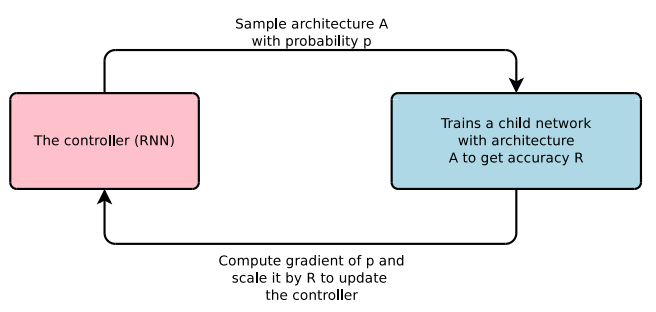
\includegraphics[width=\linewidth]{img/nas.png}
    \caption{Werking van Neural Architecture Search}
    \label{fig:nas}
\end{figure}

Dergelijke AutoML systemen gebruiken een techniek die het ontwerp van een artificieel neuraal netwerk kan automatiseren, beter bekend als Natural Architecture Search \autocite{Elsken2019}. Uit \textcite{ZophL2016} wordt vastgesteld dat deze techniek een gelijkaardige of zelfs betere performantie heeft dan modellen die door een ML-ingenieur ontworpen zijn.

Natural Architecture Search gebruikt Reinforcement Learning om een model te trainen. Deze manier van werken is fundamenteel anders dan gesuperviseerd / ongesuperviseerd leren omdat het model niet beter wordt door het gebruik van datasets. Als alternatief kan het neuraal netwerk beloningssignalen herkennen waardoor het kan leren welke acties leiden tot een positief resultaat \autocite{Lievens2019}.

Op figuur \ref{fig:nas} wordt gevisualiseerd hoe dit werkt. Op basis van controller structuur A (waarbij A een neuraal netwerk is) wordt een string met variabele lengte gegenereerd. Deze waarden worden gebruikt als parameters om een kind-netwerk aan te maken, die getraind wordt met echte data en waarbij de accuraatheid gemeten wordt aan de hand van een validatie dataset. Het resultaat wordt gebruikt als beloningssignaal voor de controller, bij de volgende iteratie kunnen er hogere kansen gegeven worden aan parameters die leiden tot accurate voorspellingen \autocite{ZophL2016}. De controller zijn zoekfunctie zal dus verbeteren over tijd.

\section{Hyperparameter tuning}

In de vorige sectie is het gebruik van parameters aan bod gekomen. Ze bepalen het gedrag van een neuraal netwerk en zijn bepalend voor het eindresultaat. Volgens \textcite{Brust2019} zijn er verschillende manieren om dit te behandelen. Brute force zal elke configuratie overlopen en beslissen hoe het model vordert terwijl feature selection gewichten aan verschillende parameters geeft. Op die manier hebben vorige simulaties een impact bij de selectie van een nieuwe set parameters \autocite{Claesen2015}.

\section{AutoML platformen}

Google Cloud AutoML zorgt voor een familiaire interface die een gebruiker snel op weg helpt. Naast Google hebben bedrijven zoals Microsoft en Amazon een platform gebouwd op hun respectievelijke cloud infrastructuur. De AutoML service kan voordelig zijn als het bedrijf al gebruik maakt van andere producten / diensten van de leverancier, extra kosten kunnen snel de lucht in gaan zonder toegang tot andere functies (bv. van Google Cloud) als dit niet het geval is. Een open source alternatief lijkt een goede oplossing, de interfaces zijn minder gebruiksvriendelijk dan een betalend product en er komt meer programmeerwerk aan te pas. Het resultaat is vaak commercieel bruikbaar zolang de restricties van de licentie gerespecteerd worden \autocite{Balter2015}. AutoKeras is een voorbeeld onder de MIT licentie, die geen commerciële restricties oplegt.
